\documentclass{article}

\usepackage[ansinew]{inputenc} %Bærbar ÆØÅ?

\usepackage{minted}
\usepackage{graphicx} % Allows figures
\usepackage{tabularx}
\usepackage{etoolbox} %for configuration of sloppy

%Section style
\usepackage{xcolor}

\definecolor{secnum}{RGB}{102,102,102}

\makeatletter
    \def\@seccntformat#1{\llap{\color{secnum}\csname the#1\endcsname\hskip 16pt}}
\makeatother
%end section style

{\sloppy}{\hbadness 10000\relax}{}{} %adds hbadness to sloppy
\setlength{\paperheight}{297mm} %Sets the page to an A4
\setlength{\paperwidth}{210mm}        %Sets the page to an A4

\begin{document}

\begin{titlepage}
\begin{center}
\textsc{Introduction to Graphics}\\[0.5cm]
\textsc{Assignment 1: Scanconversion of lines}\\[0.5cm]
\vspace{2 cm}
\begin{tabular}{ll}
Student: & Kasper Passov\\
\end{tabular}
\end{center}
\vspace{5 cm}
\newpage
\end{titlepage}

\section{Problem description}
We wish to construct an algorithm that draws a line of pixels from
point $(x1,y1)$ to $(x2,y2)$. Unfortuantly the optimal line between
these points does not always go through grid vertex's.
To combat this we design this algorithm to pick the points closest to
the optimal line.

\section{Algorithm description}

The algorithm creates a new point $d$ on the following column, halfway 
between the two pixels. The two pixels are called $\Delta E$ (The eastern one)
and $\Delta NE$ (the northeasteren one). To calculate the following point,
the line is compared to $d$, if $d$ is smaller the correct pixel is the northeastern
one, otherwise the eastern one is picked. This is then done until the of the line is
reached.

\subsection{Algorithm edgecases}

We have some different edgecases we have to keep in
mind while implementing the algorithm:

\begin{itemize}
    \item{Slope above 1}
    \item{Slope below 0}
    \item{x2 larger then x1} 
\end{itemize}

These 3 edgecases gives us a total of 8 diffrent lines that needs
to be handled.

\subsubsection{Slope above 1} This type of line I will call $y$-dominant.
It is a problem as the base algorithm always will increment the 
$x$ value, which is not correct when we have a slope above one.
It can be handlede by flipping the $x$ and $y$ coordinates of both points,
in the algorithm, while not flipping them when drawing the pixels. 
This makes the algorithm calculate the line from the perspective
of $y$ instead of $x$, and because $x$ has a slope above 1, $y$ will not

\begin{minted}{cpp}
void FltkDevice::DrawLine(int xstart, int ystart, 
                          int xend, int yend) {
    ...
    if (ydom) { //checks if y is dominat and flip values if it is
        this->DrawLineHelper(dy, dx, ystart, xstart, yend, ydom);}
    else {
        this->DrawLineHelper(dx, dy, xstart, ystart, xend, ydom);}


void FltkDevice::DrawLineHelper(int dx,  int dy, int x,   int y, 
                                int end, bool ydom) {
        ...
        if(ydom) {SetPixel(y, x, 0);} //draws ydominant pixel
            else {SetPixel(x, y, 0);}
\end{minted}

\subsubsection{Slope below 0} For this to work I need to pick the
Southeastern pixel instead of the Northeastern, I need to
decrement $y$ instead of incrementing it and when we check 0 
ageinst $d$ I have to keep in mind $\Delta SE$ should be lower then $\Delta E$. 

\begin{minted}{cpp}
void fltkdevice::drawlinehelper(int dx,  int dy, int x, int y, 
                                int end, bool ydom, bool yneg) {
    ...
    if (not yneg) {
        dNE = 2 * (dy - dx); //dNE
        dE  = 2 * dy;
        }
    else {
        ...
        % else {
            dNE = 2 * (dx - dy); //dSE
            dE  = 2 * dy;
        }
    ...
    if (yneg){checkd = (d <= 0);} // Difference between NE and SE calculations
        else {checkd = (d >  0);}
\end{minted}
Another problem emerges when we have a slope below -1. When my 
current implementation solves the problem of a slope below 0,
it flips the line upside down and uses the algorithm on the now
positive slope. This gives us the self contradicting second 
problem of having to deal with a slope that is both below 0 
and above 1. To deal with this i made a small change to the
wrapper function that deals with the y domination problems,
so that the $x$ and $y$ are not switched. 
\begin{minted}{cpp}
void FltkDevice::DrawLine(int xstart, int ystart, 
                          int xend, int yend) {
    ...
    if (ydom) { //checks if y is dominat and flip values if it is
        if (yneg) {
            int t = yend;
            yend = ystart;
            ystart = t;
            t = xend;
            xend = xstart;
            xstart = t;
            }
        this->DrawLineHelper(dy, dx, ystart, xstart, yend, ydom, yneg);}
    else {
        this->DrawLineHelper(dx, dy, xstart, ystart, xend, ydom, yneg);}
\end{minted}

\subsubsection{Negative $\Delta x$}
With a negative delta value our algorithm would have to draw from
right to left, using dW and dSW. Instead of implementing this
i used my wrapperfunction to detect this problem by comparing
$xstart$ and $xend$, and if found swap the my start and end position.
\begin{minted}{cpp}
    bool xneg = xstart > xend;

    if (xneg) { int t = xstart; xstart = xend; xend = t;
                    t = ystart; ystart = yend; yend = t;}
\end{minted}

\section{Implementation}

\begin{minted}{cpp}
void FltkDevice::DrawLine(int xstart, int ystart, 
                          int xend, int yend) {
    bool xneg = xstart > xend;

    if (xneg) { int t = xstart; xstart = xend; xend = t;
                    t = ystart; ystart = yend; yend = t;}

    bool yneg = ystart > yend;
    int dx  = xend - xstart;
    int dy  = yend - ystart;

    bool ydom = std::abs(dy) > std::abs(dx);
     
    if (ydom) { //checks if y is dominat and flip values if it is
        if (yneg) {
            int t = yend;
            yend = ystart;
            ystart = t;
            t = xend;
            xend = xstart;
            xstart = t;
            }
        this->DrawLineHelper(dy, dx, ystart, xstart, yend, ydom, yneg);}
    else {
        this->DrawLineHelper(dx, dy, xstart, ystart, xend, ydom, yneg);}
}


void FltkDevice::DrawLineHelper(int dx,  int dy, int x, int y, 
                                int end, bool ydom, bool yneg) {
    int dNE,dE;
    bool checkd;
    int d   = 2 * dy - dx;

    if (not yneg) {
        dNE = 2 * (dy - dx); //dNE
        dE  = 2 * dy;
        }
    else {
        if (ydom){
            dNE = 2 * (dy - dx); //dSE
            dE  = 2 * dx;
        }
        else {
            dNE = 2 * (dx - dy); //dSE
            dE  = 2 * dy;
        }
    }

    while (x <= end) {
        if (ydom){SetPixel(y, x, 0);} // Draws ydominant pixel
            else {SetPixel(x, y, 0);}

        if (yneg){checkd = (d <= 0);} // Difference between NE and SE calculations
            else {checkd = (d >  0);}

        if (checkd) {// Pick the NorthEast Cornor
            if (yneg){ y--;}
               else  { y++;}
        d =+ dNE;
        }
        else {
            d = d + dE;
            }
        x++;
        }
    this->Update();
    this->UnitLength(this->UnitLength(50));
}
\end{minted}

\section{Testing}
The test is generated by the following code:
\begin{minted}{cpp}
        this-> TestLine(10,5,13,6, 1.0,0.0,0.0);
        this-> DrawLine(10,5,13,6);
        this-> TestLine(9,6,10,9, 1.0,0.0,0.0);
        this-> DrawLine(9,6,10,9); //red

        this-> TestLine(10,4,13,3, 0.0,1.0,0.0);
        this-> DrawLine(10,4,13,3);
        this-> TestLine(9,3,10,0, 0.0,1.0,0.0);
        this-> DrawLine(9,3,10,0); //green

        this-> TestLine(7,4,4,3, 1.0,1.0,1.0);
        this-> DrawLine(7,4,4,3);
        this-> TestLine(8,3,7,0, 1.0,1.0,1.0);
        this-> DrawLine(8,3,7,0); //white

        this-> TestLine(7,5,4,6, 0.0,0.0,1.0);
        this-> DrawLine(7,5,4,6);
        this-> TestLine(8,6,7,9, 0.0,0.0,1.0);
        this-> DrawLine(8,6,7,9); //blue
\end{minted}
\begin{center}
    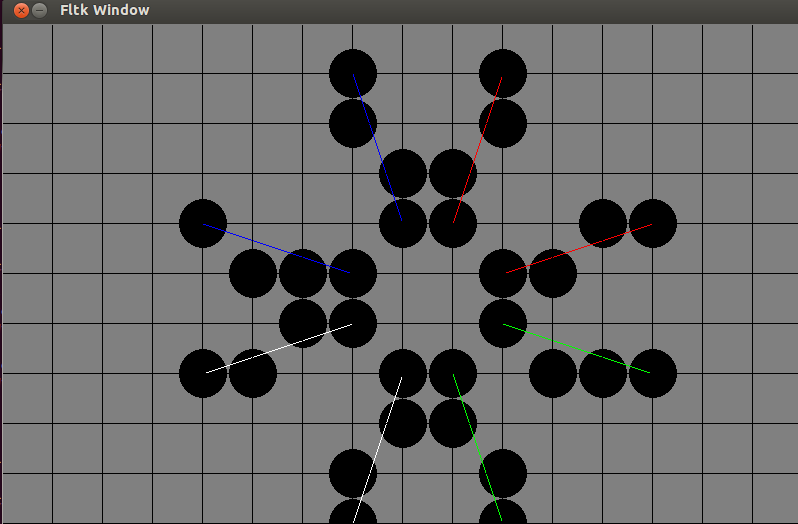
\includegraphics[scale=0.3]{GrafikTest.png}
\end{center}
As the graphic shows most of the lines works as inteded. With the
exceptions of the one with a negative slope (flat green) and its
sisterline the flat blue. I suspect this error comes from me not
finding the correct value for $\Delta SE$.

\subsection{Code}
The code for the implementation can be found in the zipped file
fltkdotdevice, and can be run with button 2.

\end{document}

